\documentclass[aagreenthesis]{subfiles}
\begin{document}
\chapter{Structure-Property in the \nfour{} Homologous Series of Molecules}

Now that the existance of the \smcpalpha{} and \smcapa{} phase have been put on
a firm footing, we can extend this study to a broad category of molecules that
share the same core, but have variations in the tail length. Our previous study
focussed on \nfour{}, with a tail length of n=14 carbons. Inspired by
previous studies by the Dublin
group\cite{SreenilayamSpontaneoushelixformation2016,SreenilayamDevelopmentferroelectricitysmectic2017,VijInvestigationheliconicalsmectic2019},
where the n16 and n18 compounds were studied and a helical phase was tentatively
determined based on periodicities of around \SI{5}{\nano\metres} see in atomic
force microscopy images.

With the ability to directly probe the periodicity of these compounds with
carbon K-edge resonant X-ray, we have the ability to provide direct evidence for
helical phases in these molecules. The high-resolution provide by RSoXS
additionally allows for a rich study of structure-property relationships, where
the nature of the helical phase can be connected to the tail-length.

Interest in the \nfour{} series of molecules is not confined to the discovery of
helicity. The additional discovery of a bent-core de Vries like phase is also a
motivating interest for study of this series. 

This chapter is organized under discussion of these two phases. First the
helical, smectic \smcpalpha{} is presented and discussed for the n12, n14, and n16 molecules.
Then the bent-core de Vries phase is presented and discussed for this series.

\section{The \smcpalpha{} Phase: Smectic Chirality Beyond the B2 Phase}


\section{The bent-core de Vries phase}

The evidence for a bent-core de Vries phase in \nfour{} will be briefly
reviewed. It is worth noting that the question of ``what is a de Vries phase''
is not settled, even for the simpler phases of rod-shaped molecules, see Jan
Lagerwall's thesis\cite{jansThesis} for an excellent history and discussion of
de Vries phases in the calamitic paradigm. For the purposes of this thesis, we
take the broadest view of a de Vries: it is a tilted phase with no long-range
order present in the tilt order parameter.

Even this broad definition is not free from ambiguity--- what entails long-range
order? We will also see in this Chapter that the de Vries phase can be
suppressed quite easily by a strong-alignment layer.



To satisfy our definition, we must prove two things about the phase under
investigation to say it is a de Vries bent-core phase. First, it must be tilted.
Second, it must have no long-range order present. Both of these facts are very
difficult to establish in a postive manner, as there is no `smoking-gun'
evidence for either.

We claim that \nfour{} is tilted for the following reasons: the smectic layer spacing is
significantly less than the extended molecular length; the lower temperature
phases are proven to be chiral (therefore tilted), and there is no observed
smectic layer-contraction observed on cooling, which would be expected for an
orthogonal$\rightarrow$ tilted phase transition; there is no measured change in the birefringence which would be predicted from an orthogonal phase to the
helical \smcpalpha{} (confirmed from RSoXS);  
The closest thing to a developed model for this phase is the Landau-de Gennes
model put forth by Eremin et al.\cite{eremin2008electrically} where they
discovered an electro-clinic analog in a hockey-stick compound. 
\todo{get and show the molecule}
\begin{figure}
    \centering
    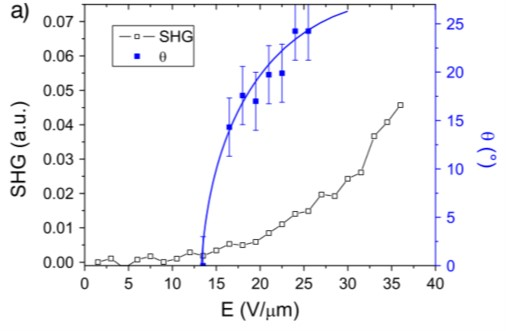
\includegraphics[width=\textwidth]{./figs/pal30/fromPapers/tiltVfield.jpg}
    \caption{\label{fig:achiralTilt} Experimental data for `hockey-stick'
    compound studied by Eremin et al.\cite{eremin2008electrically} Note, the threshold for optical tilt. The lines guide the only.}
\end{figure}
Broadly, their model describes an orthogonal bent-core phase where the polar
director is free to move. On application of an electric-field, the polarization
of the molecules orients. An enthalpic\todo{check this with ed} phase transition
is then driven by excluded-volume interactions, where the molecules can pack
more efficiently by tilting. 

This interaction is described by the following Landau-de Gennes free energy:

\begin{multline}
    f(P,\theta,T,E) = \overbrace{\left(a_0(T-T_\theta)\theta^2+b\theta^4+c\theta^6
    \right)}^{f_\theta}\\
    + \underbrace{\left( \alpha_0(T-T_P)P^2+\beta P^4 + \gamma P^6 -PE
            \right)}_{f_P} +\underbrace{\left(
    -\Gamma (P \theta)^2 \right)}_{f_{\theta P}}
\end{multline}

Though this model was originally formulated to describe the transition from an
orthogonal phase to a tilted one, we can adapt it to our bent-core de Vries
phase by changing the interpretation of $\theta$ from the molecular tilt to the
optical tilt.

Though this model succesfully captures the overall nature of the
electically-driven onset of chirality in the bent-core de Vries phase, where the
molecules first orient their polar directors to the field, and on the
achievement of total polar alignment, an optical tilt develops, it leaves much
to be desired. Because this model does not demand details of the
microscopic interactions that lead to the observed transition, there is an abundance of
fitting parameters that will lead to overfitting and the model loses most of its
predictive power.

Because of this, efforts must be undertaken to develop a microscopic model of
this de Vries phase.

\subsection{Textures of bent-code de Vries phase}

\begin{figure}[h!]
    \centering
    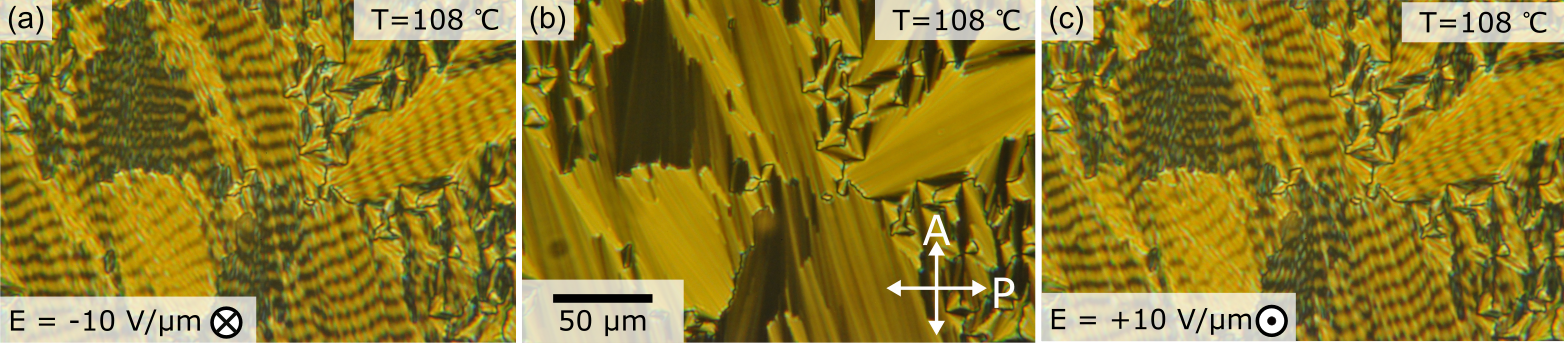
\includegraphics[width=.8\textwidth]{figs/pal30/textureSM2/sm1Textures100.png}
    \caption{\label{}}
\end{figure}


\subsection{Electro-optics of bent-core de Vries phase}
text
\begin{figure}[h!]
    \centering
    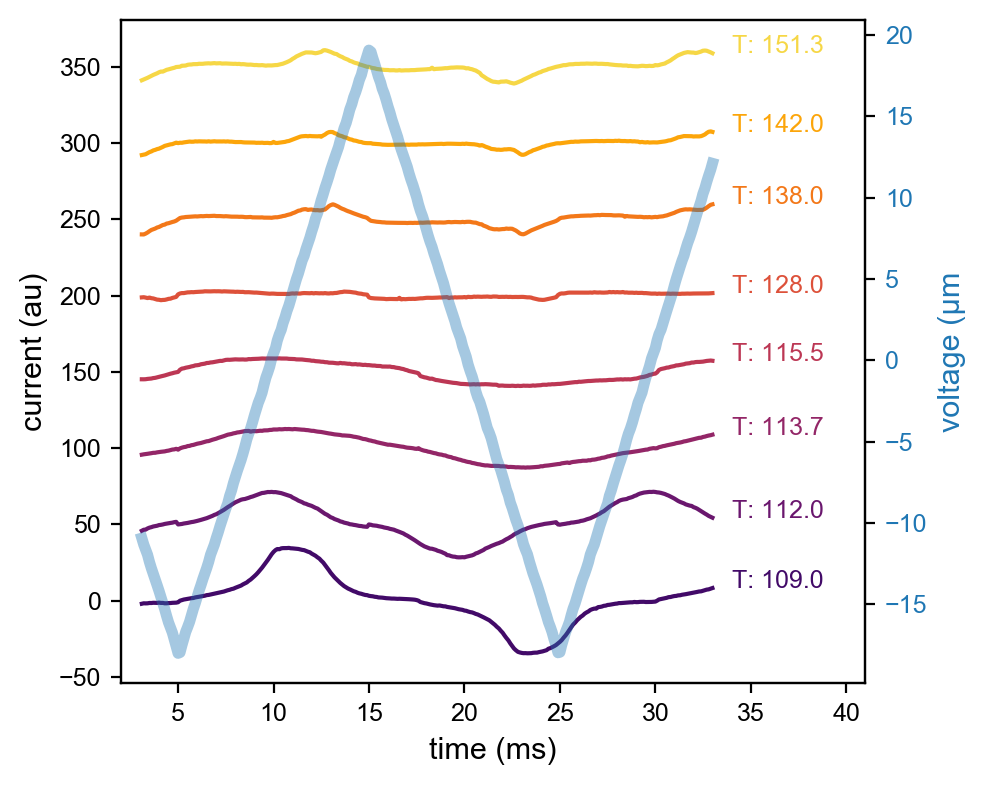
\includegraphics[width=.8\textwidth]{figs/pal30/prc/spacedSm1PRC.png}
    \caption{\label{}}
\end{figure}
text

\begin{figure}[h!]
    \centering
    \includegraphics[width=.8\textwidth]{figs/pal30/prc/3dplot-sm1.png}
    \caption{\label{}}
\end{figure}
text

\subsection{X-ray analysis of bent-core de Vries phase}

\begin{figure}[h!]
    \centering
    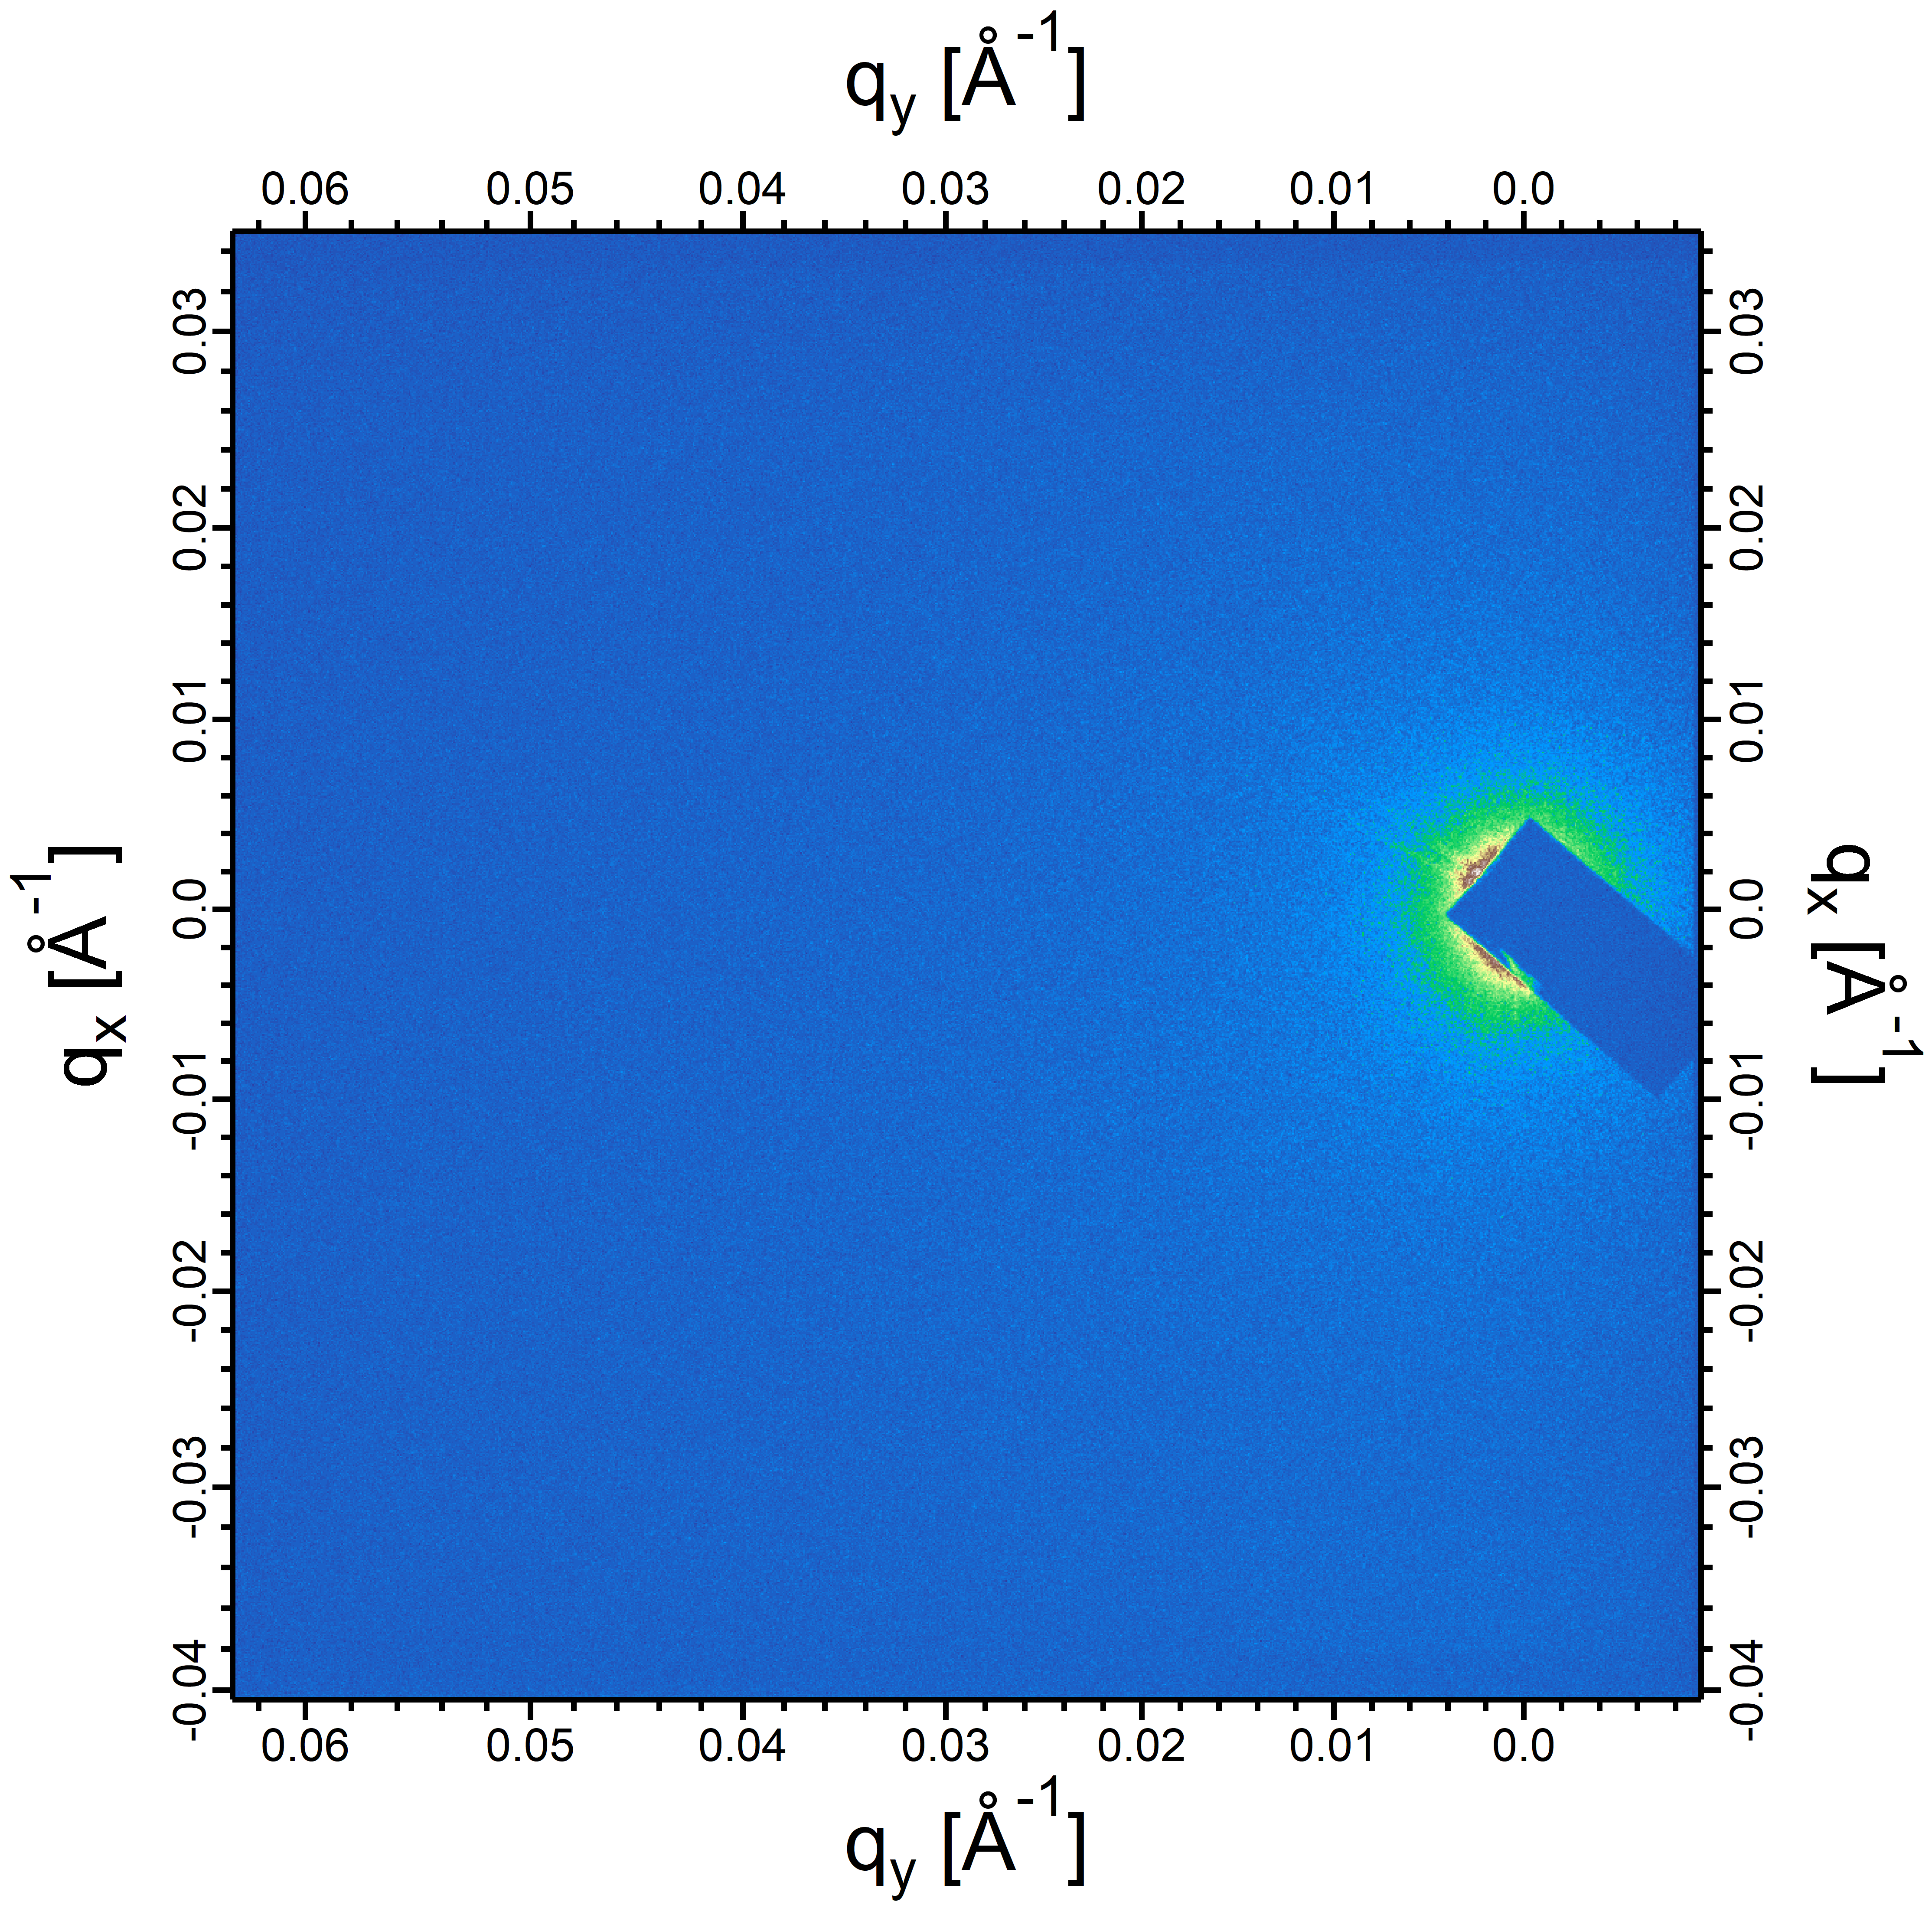
\includegraphics[width=.8\textwidth]{figs/pal30/xraysm1/rsosxSmaT113-modified.png}
    \caption{\label{}}
\end{figure}


\begin{figure}[h!]
    \centering
    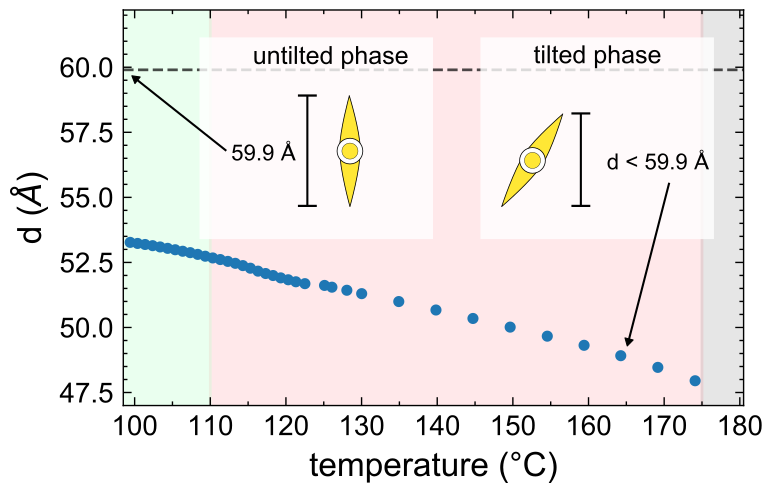
\includegraphics{figs/pal30/xraysm1/sm1-saxs-annote.png}
    \caption{\label{}}
\end{figure}




\section{Discussion for the bent-core de Vries phase}
\begin{figure}[h!]
    \centering
    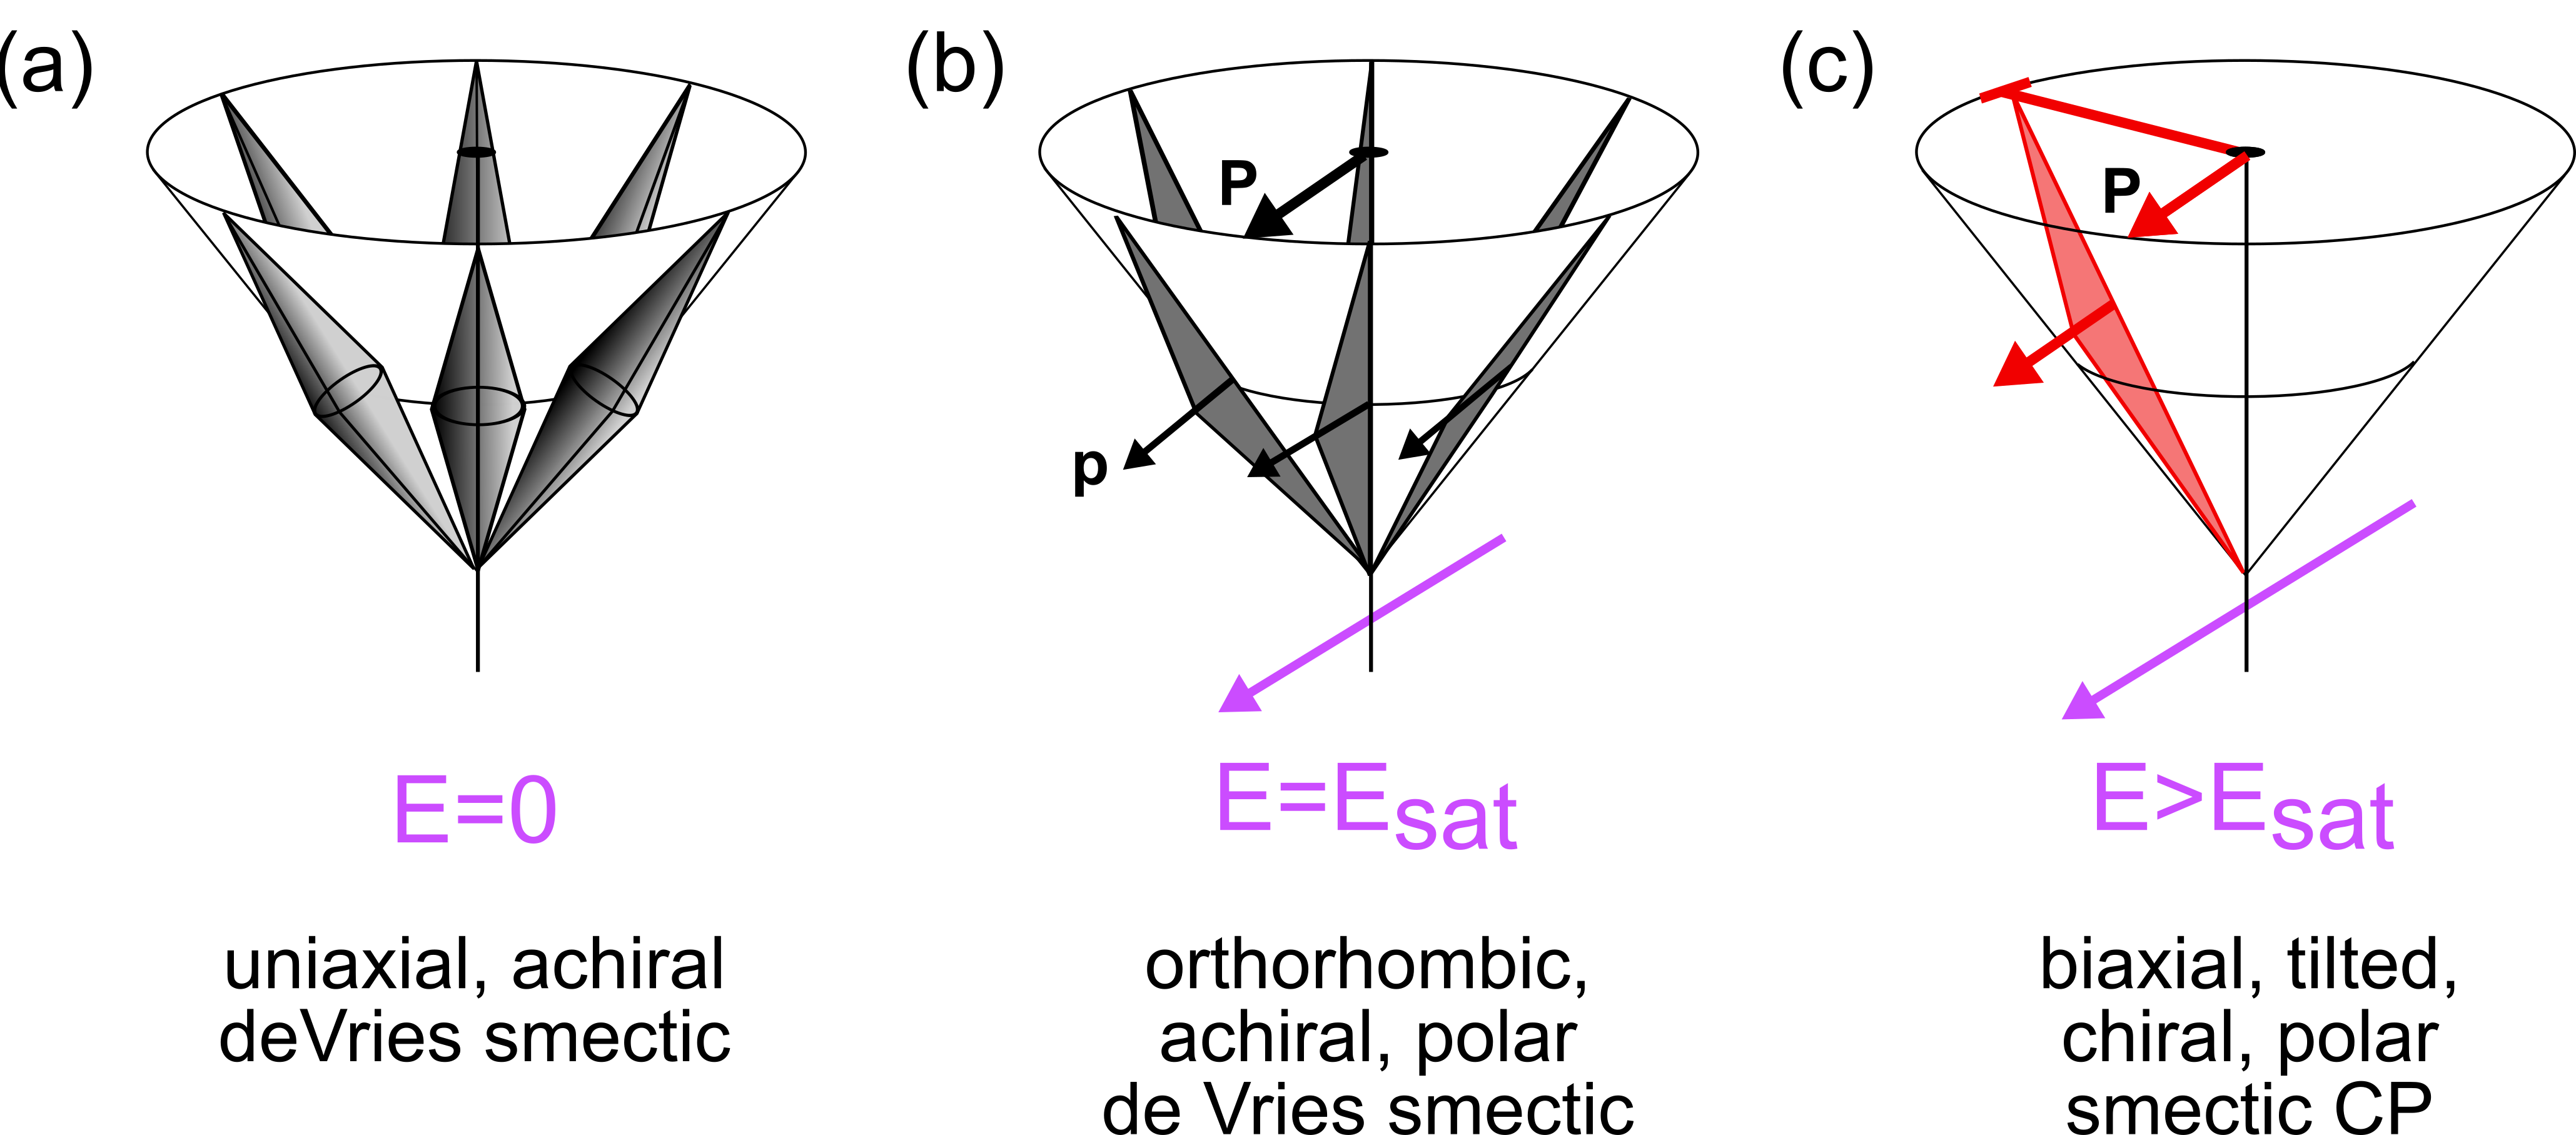
\includegraphics{figs/pal30/deVries/dvAlign.png}
    \caption{\label{}}
\end{figure}




\end{document}


